\documentclass[12pt]{standalone}
\usepackage{tikz}
\usetikzlibrary{positioning}
\begin{document}
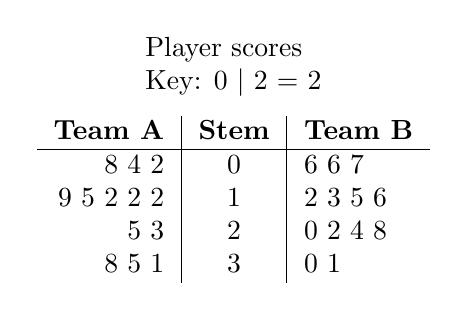
\begin{tikzpicture}
\node[align=left] (top_node) at (0,0) {Player scores \\ Key: 0 $\vert$ 2 = 2};
\node[below=of top_node,yshift=10mm] {
\begin{tabular}{r|c|l}
\textbf{Team A} & \textbf{Stem} & \textbf{Team B}\\
\hline
8 4 2 & 0 & 6 6 7 \\9 5 2 2 2 & 1 & 2 3 5 6 \\5 3 & 2 & 0 2 4 8 \\8 5 1 & 3 & 0 1 \\
\end{tabular}};
\end{tikzpicture}
\end{document}